\section{Network testing}
\textbf{Выданные параметры:} [netdev,netlink-task]
\subsection{netlink-task}
\nquote{--netlink-task N}{start  N workers that collect task statistics via the netlink taskstats interface.  This stressor can
only be run on Linux and requires CAP\_NET\_ADMIN capability.}
Найдем оптимальное количество воркеров:\\
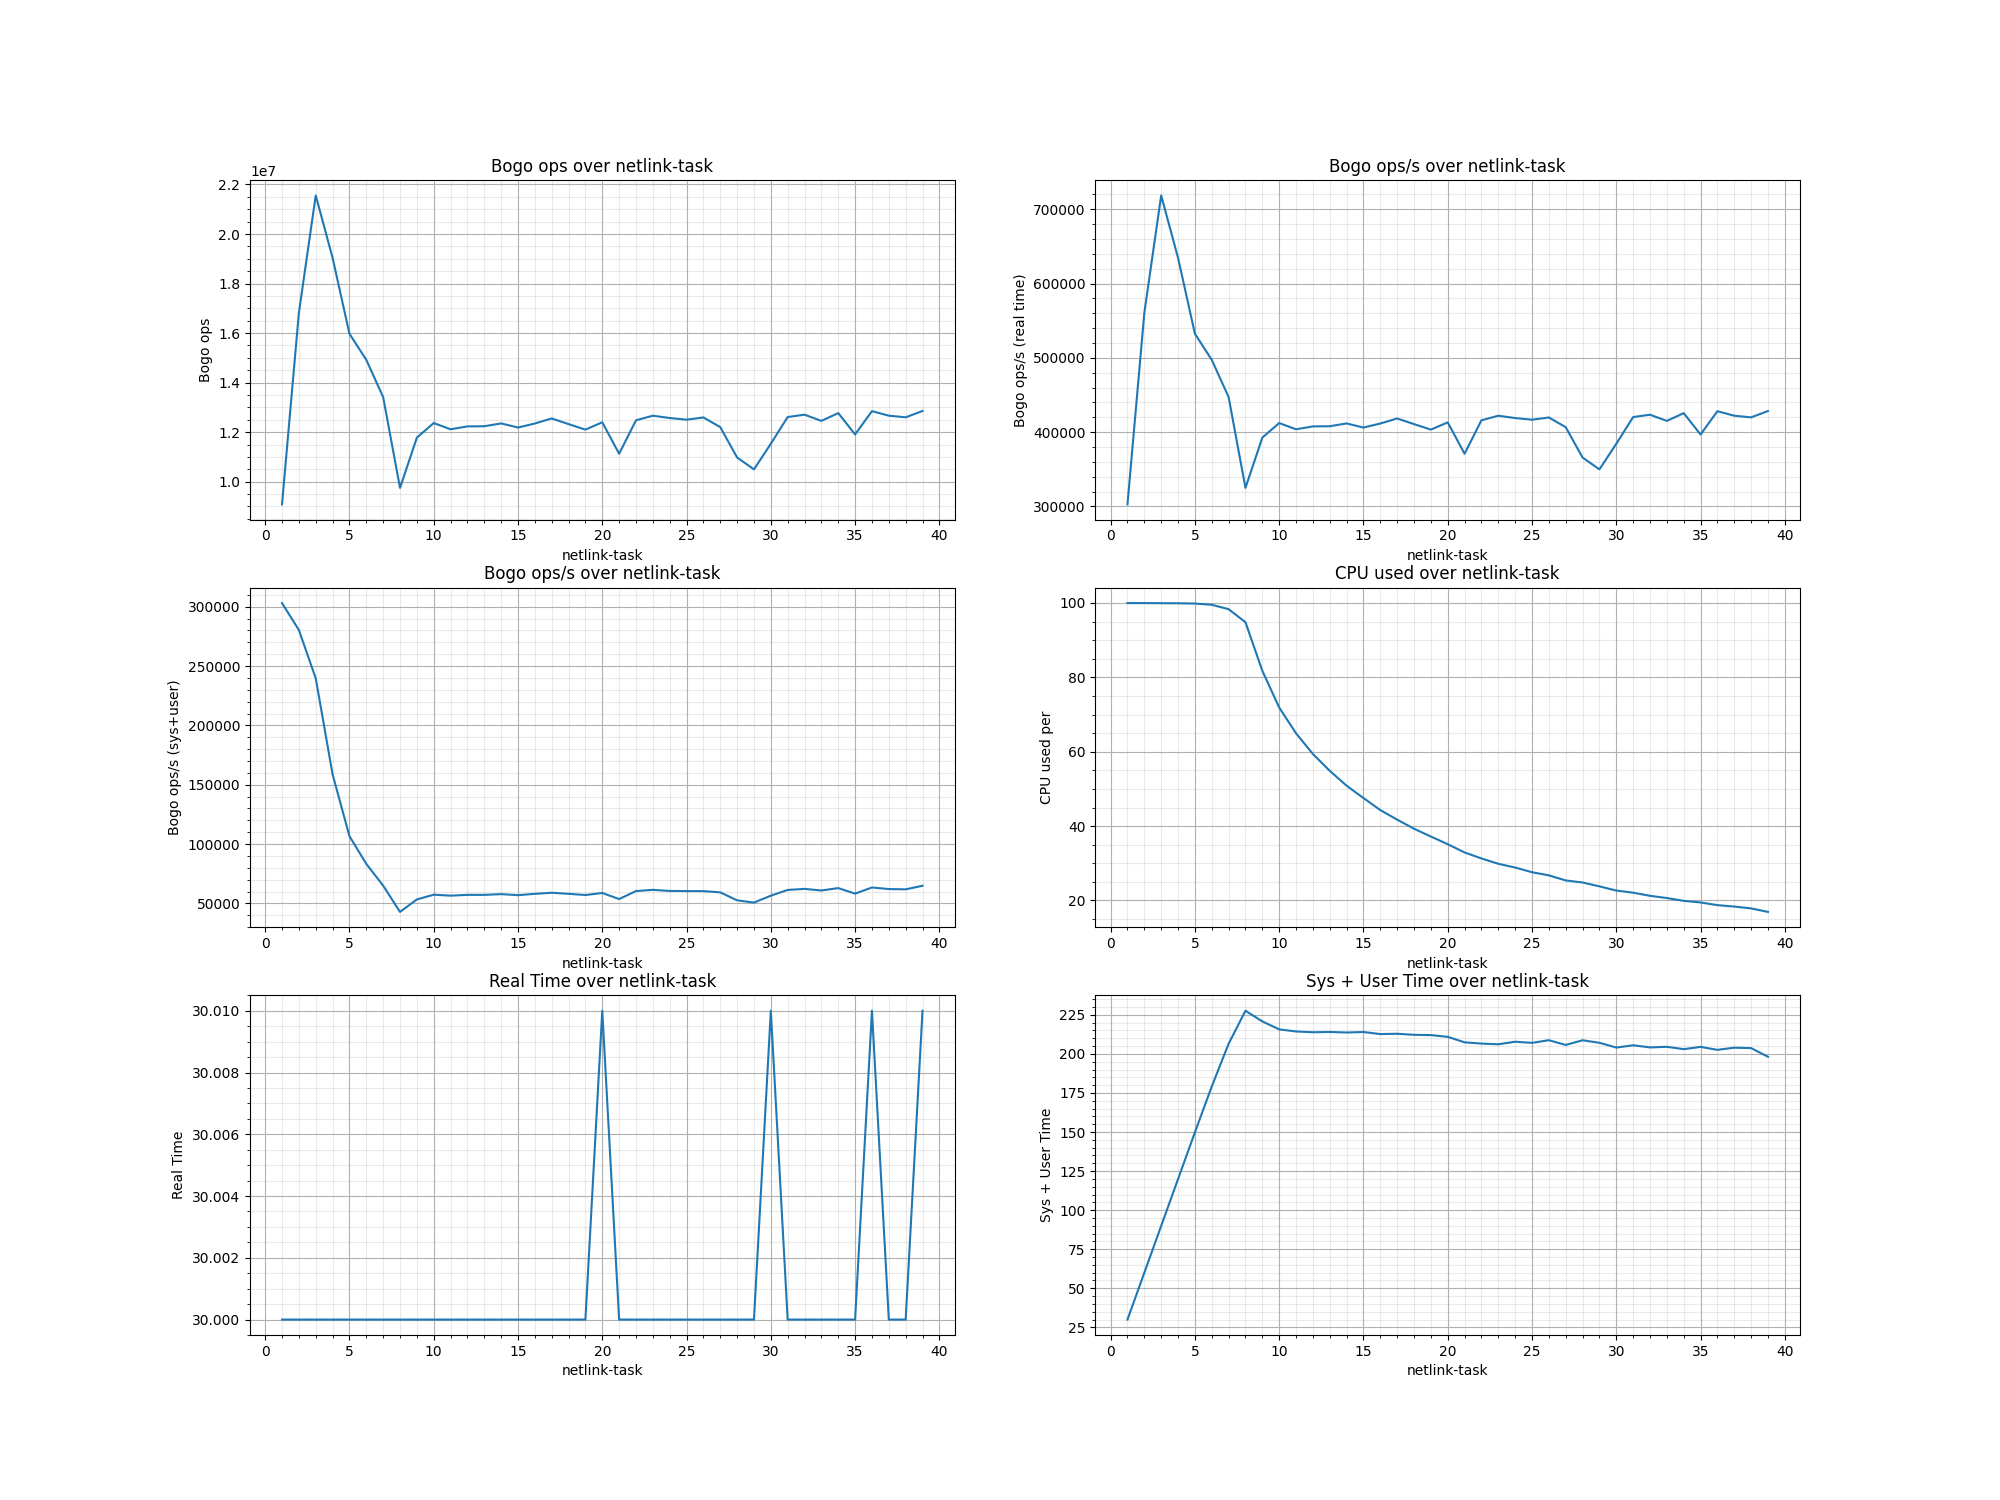
\includegraphics[width=\textwidth]{./network/image/netlink-task-bogops.png}
Максимум bogo ops достигается при 3.
\subsection{netdev}
\nquote{--netdev N}{start N workers that exercise various netdevice ioctl commands across all the available  network  devices.  The ioctls exercised by this stressor are as follows: SIOCGIFCONF, SIOCGIFINDEX, SIOCGIFNAME,
SIOCGIFFLAGS, SIOCGIFADDR, SIOCGIFNETMASK, SIOCGIFMETRIC, SIOCGIFMTU, SIOCGIFHWADDR,  SIOCGIFMAP  and
SIOCGIFTXQLEN. See netdevice(7) for more details of these ioctl commands.}
Найдем оптимальное количество воркеров:\\
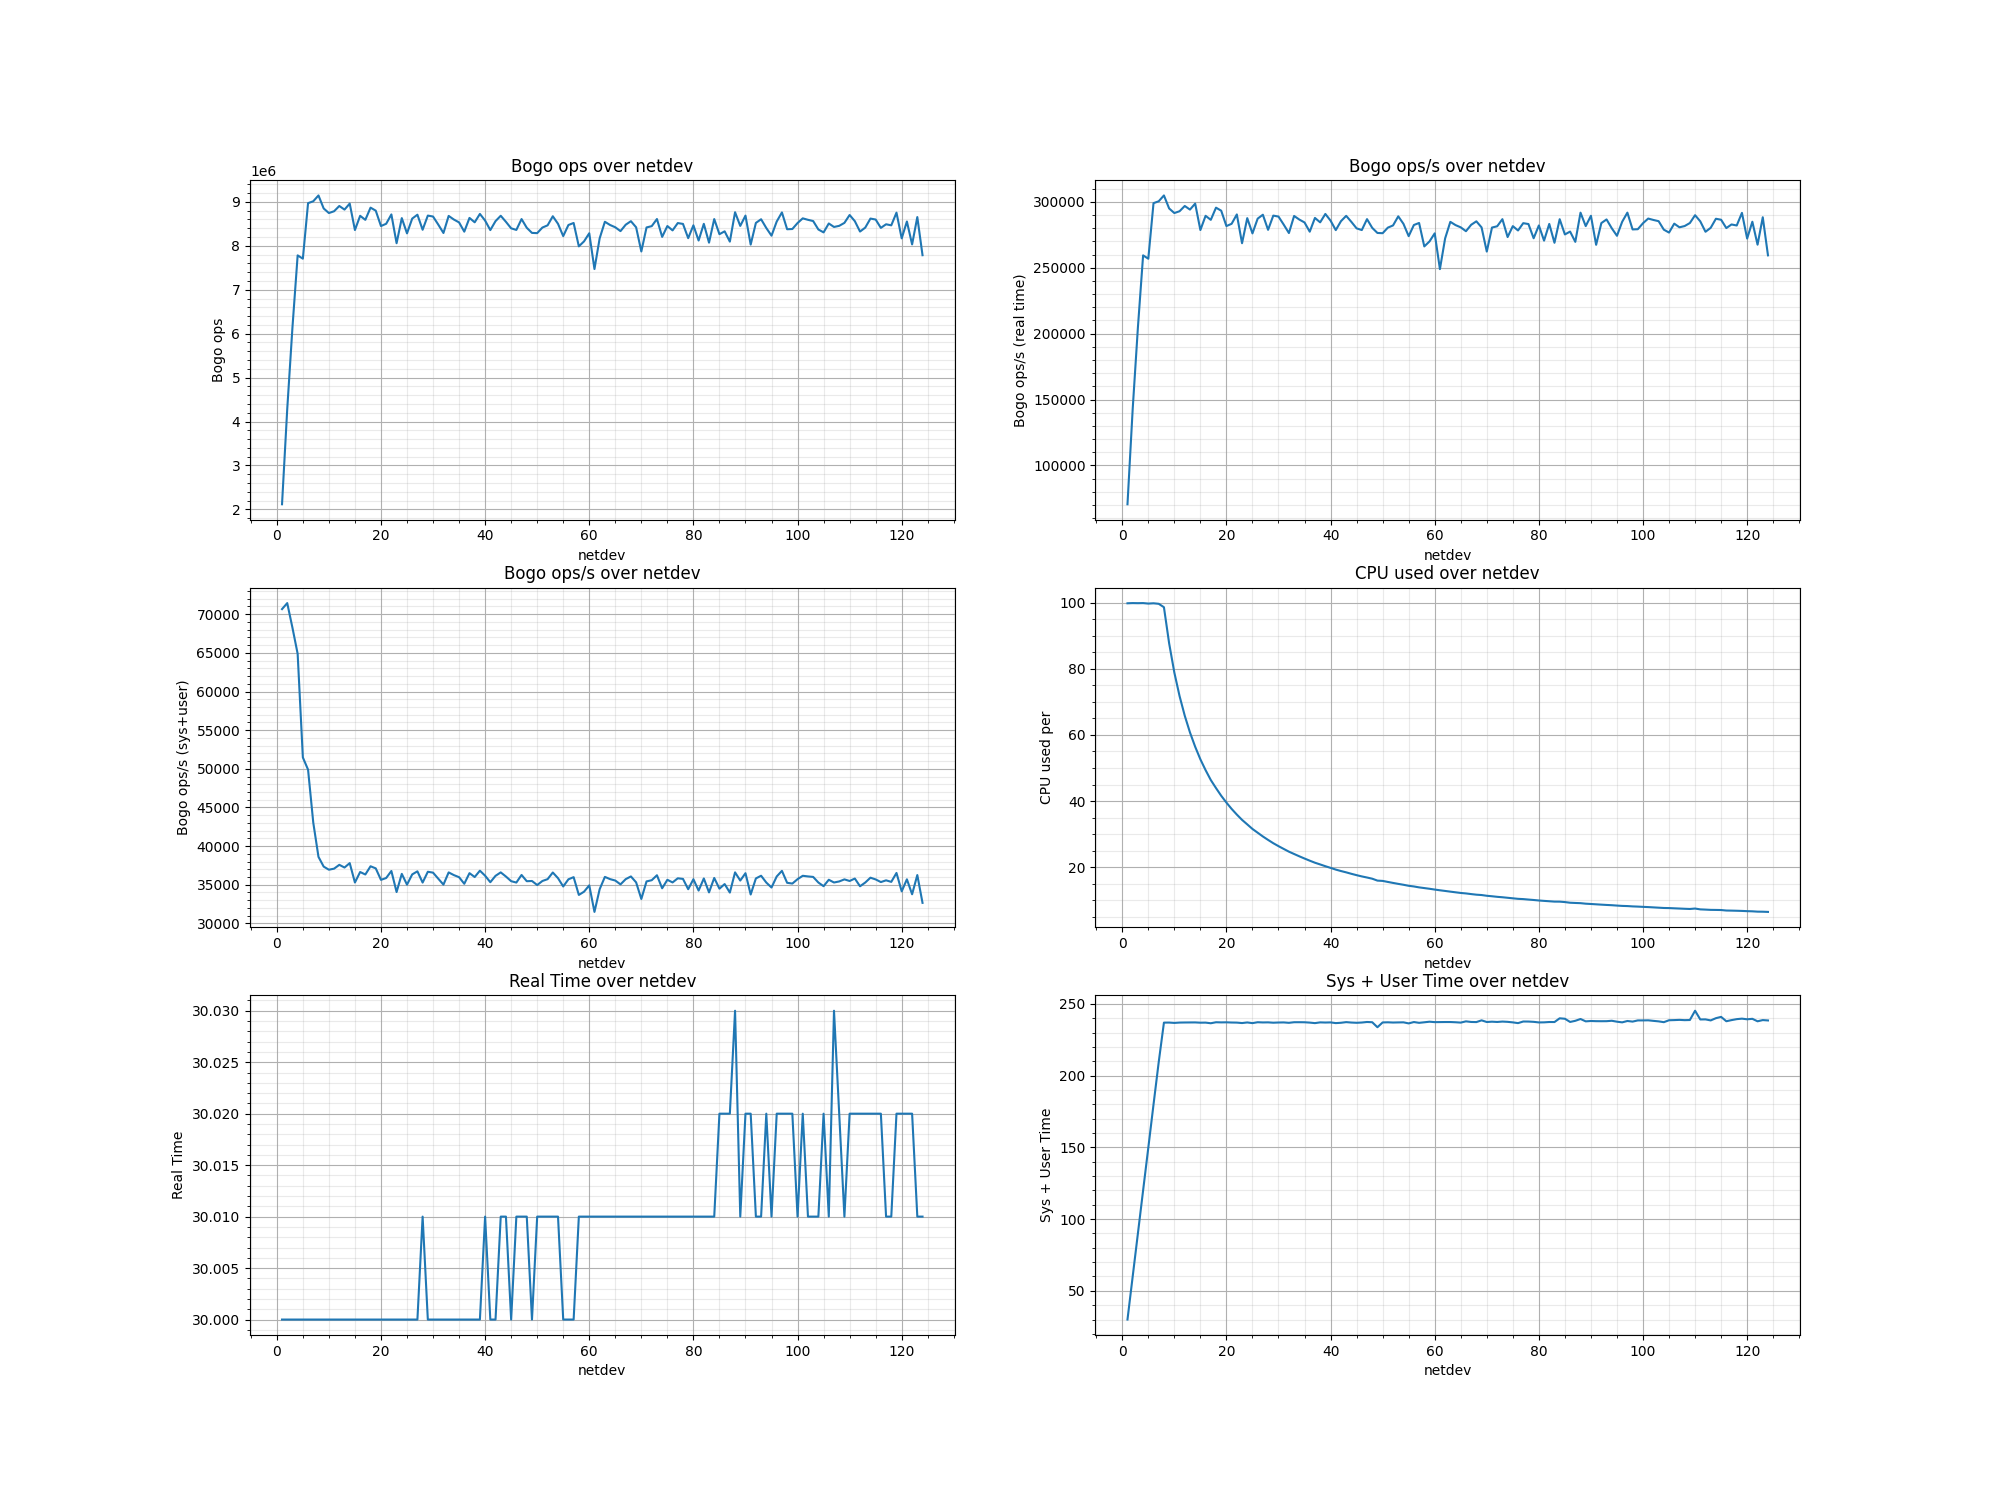
\includegraphics[width=\textwidth]{./network/image/netdev-bogops.png}
Максимум bogo ops достигается при 8.

